% VisTacFusion: original, implementation-checked, single-diagram architecture.
% Compile from paper/: pdflatex -output-directory=figures architecture_verified.tex
\documentclass[border=3pt]{standalone}
\usepackage{tikz,graphicx,amsmath,amssymb}
\usepackage{fix-cm}
\usetikzlibrary{arrows.meta,calc,backgrounds}
\definecolor{ink}{HTML}{283342}
\definecolor{tac}{HTML}{C77A3C}
\definecolor{vis}{HTML}{397FAA}
\definecolor{qry}{HTML}{7856A4}
\definecolor{bneck}{HTML}{3A8565}
\definecolor{head}{HTML}{58718E}
\tikzset{
 every node/.style={font=\sffamily\fontsize{9}{10.5}\selectfont,text=ink},
 lab/.style={font=\sffamily\fontsize{9}{10.5}\selectfont,align=center},
 title/.style={font=\sffamily\bfseries\fontsize{11}{13}\selectfont,align=center},
 box/.style={draw=ink!55,fill=white,line width=.65pt,rounded corners=2pt,
   align=center,inner sep=4pt,minimum height=.52cm},
 a/.style={draw=ink!85,line width=.75pt,-{Stealth[length=4.5pt,width=3.5pt]}},
 context/.style={a,draw=bneck,dashed},
 region/.style={rounded corners=4pt,line width=.7pt},
 op/.style={box,fill=ink!3},
}
% Token strip: seven glyphs denote a sequence (not its literal token count).
\newcommand{\strip}[4]{\begin{scope}[shift={(#1,#2)}]
 \foreach \k in {0,1,2,3,5,6}{
  \filldraw[fill=#3!22,draw=#3!85,line width=.45pt,rounded corners=.6pt]
    (\k*.19,-.12) rectangle +(.14,.24);}
 \node[lab,inner sep=0] at (.83,0) {$\cdots$};
 \coordinate (#4w) at (-.07,0); \coordinate (#4e) at (1.35,0);
\end{scope}}
\newcommand{\mapglyph}[3]{\begin{scope}[shift={(#1,#2)}]
 \filldraw[fill=tac!10,draw=tac!75,line width=.5pt] (.055,.055) rectangle +(.35,.35);
 \filldraw[fill=tac!17,draw=tac!85,line width=.5pt] (0,0) rectangle +(.35,.35);
 \draw[step=.0875,draw=tac!35,line width=.2pt] (0,0) grid (.35,.35);
 \node[lab,anchor=west] at (.46,.18) {#3};
\end{scope}}
\begin{document}
\begin{tikzpicture}[x=1cm,y=1cm]
\path[use as bounding box] (-.6,.05) rectangle (22.3,11.03);
\fill[white] (-.6,.05) rectangle (22.3,11.03);

% Regions. All are part of one connected computation graph.
\filldraw[region,draw=tac!65,fill=tac!5] (1.38,6.47) rectangle (3.75,10.82);
\filldraw[region,draw=vis!55,fill=vis!4] (6.2,6.22) rectangle (10.78,10.82);
\filldraw[region,draw=head!65,fill=head!4] (11.24,6.22) rectangle (17.25,10.82);
\filldraw[region,draw=bneck!70,fill=bneck!4] (7.00,1.15) rectangle (14.32,5.78);
\filldraw[region,draw=qry!55,fill=qry!3] (16.30,1.65) rectangle (21.88,5.78);

% Tactile backbone: four successive groups of three blocks.
\node[title] at (2.565,10.53) {SITR-B/16};
\node[lab] at (2.565,10.16) {Frozen};
\foreach \i/\y/\blocks in {1/9.5/1--3,2/8.65/4--6,3/7.8/7--9,4/6.95/10--12}{
 \node[op,draw=tac!70,text width=1.90cm] (tb\i) at (2.565,\y) {Blocks \blocks};
}
\draw[a] (tb1)--(tb2); \draw[a] (tb2)--(tb3); \draw[a] (tb3)--(tb4);
\node[inner sep=0] (it) at (.60,9.5) {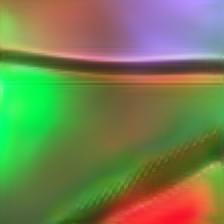
\includegraphics[width=1.04cm]{assets/tactile_sim.png}};
\node[lab] at (.60,10.30) {Tactile input};
\node[lab] at (.60,8.75) {$224\times224$};
\draw[a] (it)--(tb1.west);
\node[lab] at (4.92,10.55) {Four taps\\$196\times768$ each};

% Dense branch. Each arrow preserves one tap; the four taps are not concatenated.
\node[title] at (8.49,10.54) {Gated visual injection};
\node[lab] at (8.49,10.14) {$T'_i=T_i+\alpha_i\,\mathrm{CA}_i(T_i,B_4)$};
\node[lab] at (8.49,6.43) {$\alpha_i$ initialized to zero};
\foreach \i/\y in {1/9.5,2/8.65,3/7.8,4/6.95}{
 \strip{4.35}{\y}{tac}{t\i}
 \node[lab] at (4.98,\y+.34) {$T_{\i}$};
 \draw[a,draw=tac] (tb\i.east)--(t\i w);
 \node[box,draw=vis!70,fill=white,text width=1.93cm] (inj\i) at (7.68,\y)
  {Gated CA$_{\i}$};
 \draw[a,draw=tac] (t\i e)--(inj\i.west);
 \strip{9.11}{\y}{tac}{tp\i}
 \draw[a] (inj\i.east)--(tp\i w);
 \node[lab,anchor=east,fill=vis!4,inner sep=1pt] at (10.68,\y+.34) {$T'_{\i}$};
}

% DPT: independent reassembly -> four serial fusion operations -> shared output.
\node[title] at (14.245,10.54) {DPT decoder};
\node[lab] at (12.25,10.08) {Reassemble};
\node[lab] at (14.30,10.08) {Fusion};
\foreach \i/\y/\res in {1/9.5/56,2/8.65/28,3/7.8/14,4/6.95/7}{
 \mapglyph{11.55}{\y-.18}{$\res\times\res$}
 \draw[a] (tp\i e)--(11.46,\y);
 \node[op,text width=.93cm] (f\i) at (14.30,\y) {Fusion};
 \draw[a] (13.12,\y)--(f\i.west);
}
\draw[a] (f4.north)--node[lab,right] {$2\times$}(f3.south);
\draw[a] (f3.north)--node[lab,right] {$2\times$}(f2.south);
\draw[a] (f2.north)--node[lab,right] {$2\times$}(f1.south);
\node[box,draw=head!75,fill=head!9,text width=1.45cm,minimum height=.76cm] (shared) at (16.36,9.5)
 {Shared feature\\$112\times112$};
\draw[a] (f1.east)--node[lab,above] {$2\times$}(shared.west);
\node[lab] at (14.25,6.43) {256 feature channels};
\node[box,draw=head!75,text width=1.05cm] (dh) at (18.58,9.5) {Depth head\\$\uparrow2\times$};
\node[box,draw=head!75,text width=1.05cm] (nh) at (18.58,7.8) {Normal head\\$\uparrow2\times$};
\draw[a] (shared.east)--(dh.west);
\draw[a] (17.52,9.5)--(17.52,7.8)--(nh.west);
\fill[ink!85] (17.52,9.5) circle (.035);
\node[inner sep=0] (do) at (20.68,9.5) {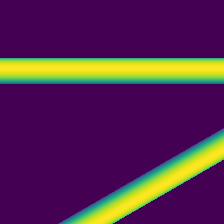
\includegraphics[width=1.17cm]{assets/depth_gt.png}};
\node[inner sep=0] (no) at (20.68,7.8) {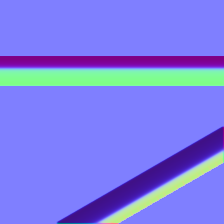
\includegraphics[width=1.17cm]{assets/normal_gt.png}};
\draw[a] (dh)--(do); \draw[a] (nh)--(no);
\node[lab] at (20.68,10.38) {Depth};
\node[lab,text width=2.5cm] at (20.68,8.63) {Surface normals};
\node[lab,text width=2.5cm] at (20.68,6.75) {Both outputs\\$224\times224$};

% Pose queries start only after the final tactile block.
\node[box,draw=tac!70,fill=tac!4,text width=1.90cm] (pt) at (2.565,5.56) {Linear\\$768\rightarrow768$};
\draw[a,draw=tac] (tb4.south)--(pt.north);
\strip{4.12}{4.70}{qry}{q0}
\filldraw[fill=qry!80,draw=qry,line width=.5pt] (5.48,4.70) circle (.105);
\node[lab] at (4.80,5.25) {Queries $Q_0$};
\node[lab] at (4.80,4.08) {196 spatial + 1 pose\\$197\times768$};
\draw[a] (pt.south)--(2.565,4.7)--(q0w);

% Visual branch. M is an independent input, never concatenated with Q.
\node[inner sep=0] (iv) at (.6,2.7) {
\includegraphics[width=1.04cm]{assets/rgb_sim.png}};
\node[lab] at (.6,3.51) {Visual input};
\node[lab] at (.6,1.95) {$224\times224$};
\node[box,draw=vis!75,fill=vis!5,text width=1.82cm,inner sep=3pt] (ev) at (2.565,2.7)
 {\textbf{MAE-L/16}\\24 blocks\\Frozen};
\draw[a] (iv)--(ev);
\node[box,draw=vis!75,text width=1.70cm,inner sep=1pt] (pv) at (4.55,2.7) {Linear\\$1024\!\to\!768$};
\draw[a,draw=vis] (ev)--(pv);
\strip{5.60}{2.70}{vis}{mem}
\draw[a,draw=vis] (pv.east)--(memw);
\node[lab] at (6.23,3.45) {Visual memory $M$};
\node[lab,text width=2.30cm] at (6.23,1.91) {$197\times768$\\Read-only};

% A fusion layer is shown once and repeated four times with carried states.
\node[title] at (10.66,5.49) {Asymmetric fusion\; $\times4$ layers};
\node[op,text width=1.25cm] (cqb) at (8.07,4.7) {Cross-attn};
\node[op,text width=.60cm] (ff1) at (9.75,4.7) {FFN};
\node[op,text width=1.20cm] (sa) at (11.40,4.7) {Self-attn};
\node[op,text width=.60cm] (ff2) at (13.03,4.7) {FFN};
\draw[a,draw=qry] (5.67,4.7)--node[lab,above] {$Q_{\ell-1}$}(cqb.west);
\draw[a] (cqb)--(ff1);
\draw[a] (ff1)--node[lab,above] {$\widetilde Q_\ell$}(sa);
\draw[a] (sa)--(ff2);
\node[op,text width=1.25cm] (cbb) at (8.07,2.7) {Cross-attn};
\draw[a,draw=vis] (meme)--node[lab,above] {K,V}(cbb.west);
\node[lab] (bp) at (8.07,1.83) {$B_{\ell-1}$};
\draw[a,draw=bneck] (bp.north)--node[lab,right] {Q}(cbb.south);
\strip{9.47}{2.70}{bneck}{bl}
\draw[a,draw=bneck] (cbb.east)--(blw);
\node[lab] at (10.10,2.25) {$B_\ell$: 16 tokens};
\draw[context] (10.10,2.82)--(10.10,3.62)--(8.07,3.62)--node[lab,left] {K,V}(cqb.south);
\node[lab,text width=6.80cm] at (10.66,1.43) {Learned $B_0$; carry $B_\ell$ and $Q_\ell$ to the next layer.};
\node[lab] at (10.30,.83) {Attention and FFN sublayers include pre-normalization and residual connections.};

% Final B4 is the sole visual context for dense injection.
\strip{12.49}{2.70}{bneck}{b4}
\draw[a,draw=bneck] (ble)--node[lab,above,align=center] {final\\layer}(b4w);
\node[lab] at (13.12,3.19) {$B_4$};
\node[lab] at (13.12,2.23) {$16\times768$};
\draw[context] (b4e)--(14.85,2.7)--(14.85,6.00)--(8.49,6.00)--(8.49,6.22);
\node[lab,fill=white,inner sep=2pt] at (11.45,6.00) {$B_4$: K,V for all four taps};

% Query output crosses the conditioning line with an explicit bridge (no junction).
\draw[a,draw=qry] (ff2.east)--(14.68,4.7) to[out=65,in=115] (15.02,4.7)--(15.11,4.7);
\node[lab] at (14.00,5.01) {$Q_\ell$};
\strip{15.18}{4.70}{qry}{q4}
\node[lab] at (15.78,5.25) {$Q_4$};

% Both pose and spatial tokens are selected from Q4, never from B4.
\node[title] at (19.09,5.49) {Pose head};
\coordinate (split) at (16.65,4.70);
\draw[draw=qry,line width=.75pt] (q4e)--(split);
\fill[qry] (split) circle (.035);
\node[circle,draw=qry,fill=qry!80,minimum size=.22cm,inner sep=0] (p4) at (17.30,4.70) {};
\draw[a,draw=qry] (split)--(p4);
\node[lab,anchor=west] at (17.60,4.86) {$p_4$ (768)};
\strip{16.86}{2.85}{qry}{qs}
\draw[a,draw=qry] (split)--(16.65,2.85)--(qsw);
\node[lab,text width=1.50cm] at (17.49,3.43) {Spatial\\tokens};
\node[box,text width=1.38cm] (mean) at (19.16,2.85) {MeanPool\\768};
\draw[a] (qse)--(mean.west);
\node[box,text width=1.10cm] (cat) at (19.16,4.05) {Concat\\1536};
\draw[a] (p4.south)--(17.30,4.05)--(cat.west);
\draw[a] (mean.north)--(cat.south);
\node[box,draw=qry!65,text width=.90cm] (mlp) at (21.02,4.05) {Pose MLP};
\draw[a] (cat)--(mlp);
\node[lab,text width=2.00cm] (poseout) at (21.00,2.73) {Planar pose\\$(\cos\theta,\sin\theta)$\\$(t_x,t_y)$};
\draw[a] (mlp.south)--(poseout.north);
\node[lab] at (19.09,1.96) {$[\,p_4\;\Vert\;\operatorname{mean}(Q_4^{\mathrm{sp}})\,]$};

% Compact legend; symbolic token counts and omitted embeddings are in the caption.
\node[lab,anchor=west] at (.10,.42) {
 \textcolor{tac}{\rule{7pt}{7pt}} Tactile\quad
 \textcolor{vis}{\rule{7pt}{7pt}} Visual\quad
 \textcolor{qry}{\rule{7pt}{7pt}} Queries\quad
 \textcolor{bneck}{\rule{7pt}{7pt}} Bottlenecks};
\node[lab,anchor=east] at (21.85,.42) {Paired inputs shown; batch dimensions omitted.};
\end{tikzpicture}
\end{document}
